\documentclass[a4paper]{article}

\usepackage{amssymb,,hyperref,graphicx}

\title{Assignment 3 - Question 4}
\author{Ory Band \texttt{300479425}}
\date{\today}

\newtheorem{thm}{Theorem}

\usepackage{fancyhdr}
\pagestyle{fancy}
\lhead{Ory Band \texttt{300479425}}
\rhead{}
\renewcommand{\headrulewidth}{0.4pt}
\renewcommand{\footrulewidth}{0.4pt}

\begin{document}

\maketitle
\newpage

\section {Question 4}

\subsection {Perceptron}

To test the perceptron, I generated 10,000 samples in $\mathbb{R}^2$,
bounded by a 1-radius circle.
The data set was split 7500/2500 for training/testing respectively.
\\
\\
At first I tested on a completely seperable data set: Every sample above
a certain threshold (upper diagonal) was marked as positive,
and everything below that as negative.
The perceptron learned very quickly (only 2 iterations), with 100\% success.

\begin{figure}[h!]
    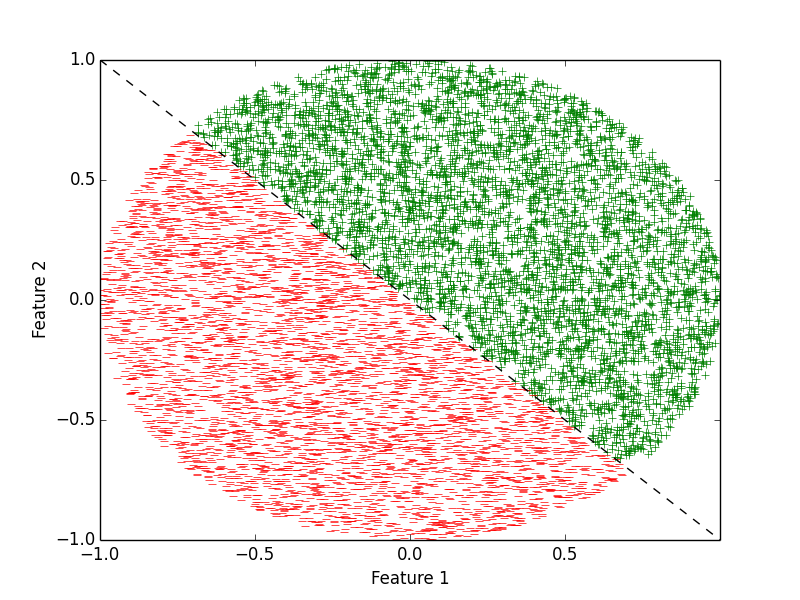
\includegraphics[width=1.0\textwidth]{images/seperable.png}
\end{figure}

\newpage

Afterwards I regenerated the data set, and set all samples within a band of
1.4 thickness to be randomly positive or negative. I tested the success rate
as a function of an increasing training data set, from 1500 to 7500,
with a bound of 1000 iterations per size, and a learning rate of 0.01.
\\
\\
All sizes resulted in a 65-70\% success rate, explained by the inseperable data.

\begin{figure}[h!]
    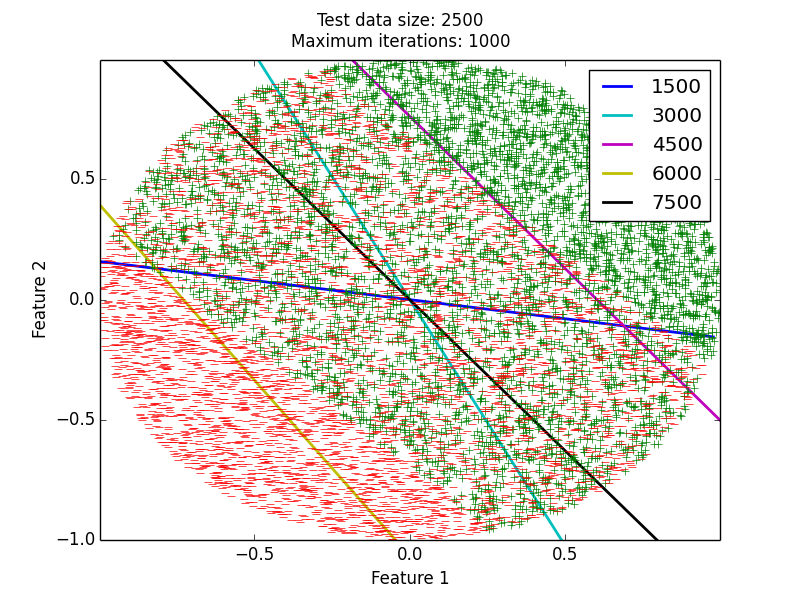
\includegraphics[width=1.0\textwidth]{images/inseperable.png}
    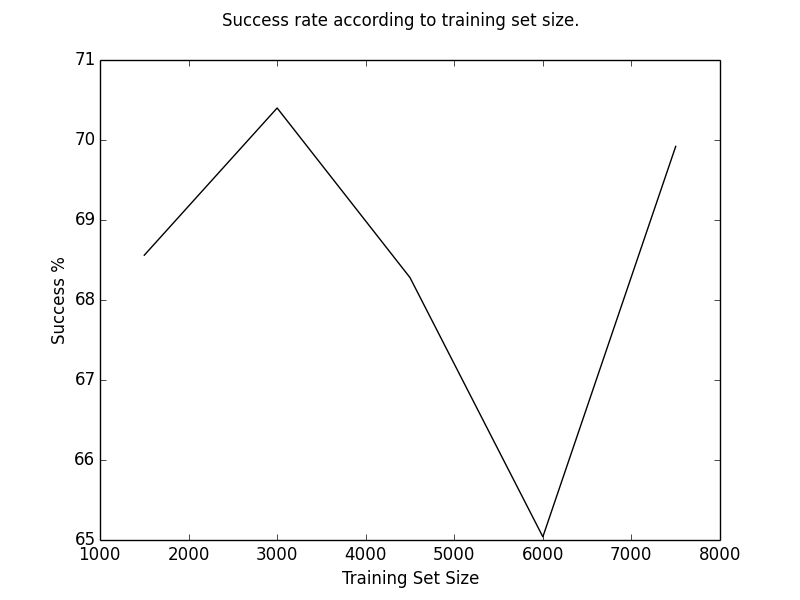
\includegraphics[width=0.8\textwidth]{images/success_rate.png}
\end{figure}

\newpage

\subsection {Skin Segmentation}

Afterwards, I tested the perceptron on UCI's skin segmentation data set.
data set.
Data was in $\mathbb{R}^3$, and seemed pretty much seperable according to the results.
\\
URL: \url{https://archive.ics.uci.edu/ml/datasets/Skin+Segmentation}
\\
\\
I tested twice with an increasing data set over 10 steps,
once with a bound of 300 iterations, and then with a bound of 1000.
\end{document}
